\documentclass[a4paper,11pt]{article}
\usepackage{amsmath,amsthm,amsfonts,amssymb,amscd,amstext,vmargin,graphics,graphicx,tabularx,multicol} \usepackage[french]{babel}
\usepackage[utf8]{inputenc}  
\usepackage[T1]{fontenc} 
\usepackage[T1]{fontenc}
\usepackage{amsmath,amssymb}
\usepackage{pstricks-add,tikz,tkz-tab,variations}
\usepackage[autolanguage,np]{numprint} 
\usepackage{enumitem}

\setmarginsrb{1.5cm}{0.5cm}{1cm}{0.5cm}{0cm}{0cm}{0cm}{0cm} %Gauche, haut, droite, haut
\newcounter{numexo}
\newcommand{\exo}[1]{\stepcounter{numexo}\noindent{\bf Exercice~\thenumexo} : \marginpar{\hfill /#1}}
\reversemarginpar


\newcounter{enumtabi}
\newcounter{enumtaba}
\newcommand{\q}{\stepcounter{enumtabi} \theenumtabi.  }
\newcommand{\qa}{\stepcounter{enumtaba} (\alph{enumtaba}) }
\newcommand{\initq}{\setcounter{enumtabi}{0}}
\newcommand{\initqa}{\setcounter{enumtaba}{0}}

\newcommand{\be}{\begin{enumerate}}
\newcommand{\ee}{\end{enumerate}}
\newcommand{\bi}{\begin{itemize}}
\newcommand{\ei}{\end{itemize}}
\newcommand{\bp}{\begin{pspicture*}}
\newcommand{\ep}{\end{pspicture*}}
\newcommand{\bt}{\begin{tabular}}
\newcommand{\et}{\end{tabular}}
\renewcommand{\tabularxcolumn}[1]{>{\centering}m{#1}} %(colonne m{} centrée, au lieu de p par défault) 
\newcommand{\tnl}{\tabularnewline}

\newcommand{\trait}{\noindent \rule{\linewidth}{0.2mm}}
\newcommand{\hs}[1]{\hspace{#1}}
\newcommand{\vs}[1]{\vspace{#1}}

\newcommand{\N}{\mathbb{N}}
\newcommand{\Z}{\mathbb{Z}}
\newcommand{\R}{\mathbb{R}}
\newcommand{\C}{\mathbb{C}}
\newcommand{\Dcal}{\mathcal{D}}
\newcommand{\Ccal}{\mathcal{C}}
\newcommand{\mc}{\mathcal}

\newcommand{\vect}[1]{\overrightarrow{#1}}
\newcommand{\ds}{\displaystyle}
\newcommand{\eq}{\quad \Leftrightarrow \quad}
\newcommand{\vecti}{\vec{\imath}}
\newcommand{\vectj}{\vec{\jmath}}
\newcommand{\Oij}{(O;\vec{\imath}, \vec{\jmath})}
\newcommand{\OIJ}{(O;I,J)}

\newcommand{\bmul}[1]{\begin{multicols}{#1}}
\newcommand{\emul}{\end{multicols}}


\newcommand{\reponse}[1][1]{%
\multido{}{#1}{\makebox[\linewidth]{\rule[0pt]{0pt}{20pt}\dotfill}
}}

\newcommand{\titre}[5] 
% #1: titre #2: haut gauche #3: bas gauche #4: haut droite #5: bas droite
{
\noindent #2 \hfill #4 \\
#3 \hfill #5

\vspace{-1.6cm}

\begin{center}\rule{6cm}{0.5mm}\end{center}
\vspace{0.2cm}
\begin{center}{\large{\textbf{#1}}}\end{center}
\begin{center}\rule{6cm}{0.5mm}\end{center}
}



\begin{document}
\pagestyle{empty}
\titre{TicTacToe sur Scratch}{}{
\includegraphics[scale=0.2]{tictac.eps}}{}{5eme}



\textbf{{\large Écrire un programme avec Scratch.}} 

Un programme est constitué de scripts, qui dirigent le comportement d'objets graphiques (appelés « lutins » dans
Scratch), qui peuvent se déplacer, être actifs, ou non. 

Les scripts s'écrivent en emboîtant des « briques » de différentes couleurs.

Pour écrire un script, il suffit de faire glisser les briques depuis la zone des briques vers la zone des scripts. 

Les briques s'emboîtent alors comme dans un puzzle, pour créer des instructions.\\


\medskip

\begin{flushleft}
\includegraphics[scale=1.3]{jeu1.eps} 
\end{flushleft}

{\large \textbf{Les différentes étapes}}\\

Programmer un jeu de type « TicTacToe ».

\bi
\item Défi 1 : Création d'une grille de TicTacToe sur la scène
\item Défi 2 : Création de deux joueurs qui se déplacent 
\item Défi 3 : Création des motifs respectifs au 2 joueurs
\item Défi 4 : Tester le jeu et proposer des améliorations
\ei

\newpage

\textbf{{\large \begin{center}
Défi 1 – Créer une grille de TicTacToe sur la scène.
\end{center}}}

\noindent Pour cela il suffit de cliquer sur l'outil  "Scène" puis "arrière-plans" et d'utiliser l'outil ligne pour dessiner la grille que vous souhaitez.


\begin{flushleft}
\includegraphics[scale=0.7]{scene1.eps} 
\end{flushleft}





\vspace*{1cm}

\textbf{{\large \begin{center}
Défi 2 – Déplacement des joueurs
\end{center}}}

Vous allez créer deux personnages qui se déplaceront à l'écran. Ils pourront se déplacer dans les 4 directions (droite, gauche,
haut, bas) à l'aide des flèches du clavier  ou d'autres touches (par exemple : les lettres Q,Z,S,D).\\

\underline{\textbf{Étape 1} }: Déplacement du joueur vers la droite.\\

\noindent 1. L'onglet « Script » est sélectionné.\\
2. Cliquer sur le bouton « Évènements » (bord marron).\\
3. Faire glisser la brique marron « quand espace est cliqué » vers la zone de script.\\
4. Cliquer sur la petite flèche à côté de « espace » et choisis « flèche droite »\\
5. Cliquer sur le bouton « Mouvement » (bord bleu), et fais glisser la brique bleue « s'orienter à 90 » vers la zone de script.\\
6. Emboîter la brique « s'orienter à 90 » et la brique « quand flèche droite est pressée ».\\
7. Faire glisser la brique bleue « avancer de 10 pas » vers la zone de script.\\
8. Emboîter la brique « avancer de 10 pas » avec la brique « s'orienter à 90 ».\\
9. Appuyer sur la flèche droite du clavier, et regarder le personnage aller vers la droite.\\

\underline{\textbf{Étape 2}} : Déplacement du joueur vers la gauche\\

\noindent 10. Répéter les mêmes étapes que pour l'étape 1.\\
11. Appuyer sur la flèche gauche du clavier, et regarder le joueur 1 aller vers la gauche.\\
12. Problème : il a la tête en bas. Pour y remédier afficher le menu contextuel du joueur 1, avec le bouton droit de
la souris, et sélectionne « info » (Repère 1) . Choisir le style de rotation 
\includegraphics[scale=1]{fleche.eps} ,  retournement gauche/droite uniquement.\\

\includegraphics[scale=1]{jeu2.eps} \\

\underline{\textbf{Étapes 3 et 4}} : Faire aller le joueur dans les 2 autres directions.\\

\noindent 13. Compléter le script pour que le joueur puisse être déplacé vers le haut et vers le bas, avec les flèches haut et bas du clavier.\\

Il ne reste plus qu'à faire de même avec l'autre joueur.\\


\textbf{$\rightarrow$ Ne pas oublier de sauvegarder le programme en l'enregistrant dans l'espace de travail sur le serveur du collège.
(Fichier - Enregistrer sous - ordinateur - Devoirs - Nomprénom ...)}\\


\textbf{{\large \begin{center}
Défi 3 – Création des motifs respectifs aux deux joueurs
\end{center}}}

Dans la zone de script du joueur 1 et 2, ajouter les briques ci-dessous. \\

\begin{center}

\includegraphics[scale=1]{dessin.eps} \hspace*{2cm}
\includegraphics[scale=1.1]{dessin2.eps} 
\end{center}



Et compléter en ajoutant les briques nécessaires au dessin de leur motif (carré, rectangle, triangle, croix, ...).\\

\textbf{{\large \begin{center}
Défi 4 – Test et améliorations
\end{center}}}

Tester votre jeu avec un camarade et proposer des améliorations pour le perfectionner.\\

Faîtes évoluer votre jeu avec : un écran de début, un écran de fin, en mettant des sons à certains moments, en comptant les points ...\\

\textbf{$\rightarrow$ Ne pas oublier de sauvegarder le programme en l'enregistrant dans l'espace de travail sur le serveur du collège.
(Fichier - Enregistrer sous - ordinateur - Devoirs - Nomprénom ...)}\\
\end{document}
